\documentclass{article}
\usepackage{geometry}
\usepackage{graphicx}
\usepackage{setspace}

% Title
\title{Wifi Connected Chess Boards \\ \large Design Specification}
\author{Nick Kraus, Kyle Jameson, Maurice Wallace, Mark Mauriello}
\date{\today}

% Margins
\geometry{letterpaper, portrait, margin=.75in}

% Double Spaced
\doublespacing

\begin{document}

\maketitle

\section*{Summary}
\indent

The State diagram overlaps the activity of both players 1 and 2 before a game of chess commences. Both players initialize their chess boards and connect to the server using the IP address input given by the microcontroller. With this, a game has commenced and player 2 waits for player 1 to complete his move. Once player 1 makes his play, the legality of the move will be evaluated. If the move is illegal, the user is warned of the play and then prompted to make a second move, through the LCD display. If a move is legal, it is sent to the server. With this, the current players turn is over and then begins to wait for his opponent to continue the game. In the event that a move is both legal and triggers a checkmate, the game is over. While waiting for his turn player 2's board will query the server to see if it has a move waiting. If a move is pending it will be sent to the board which will then move the pieces to the correct location, and wait for player 2 to make their move.

\vspace*{5mm}

\centerline{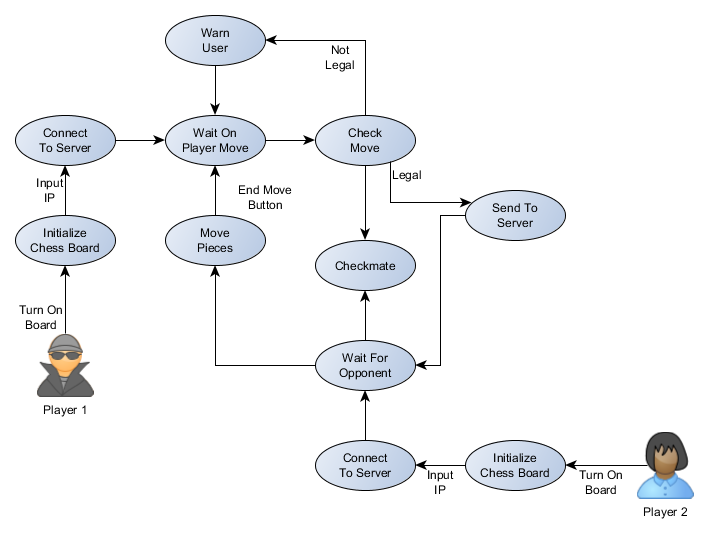
\includegraphics[scale=.5]{High_Level_State}}

\begin{center}
State diagram of the overall system, including the two users.
\end{center}

\vspace*{5mm}
	
\section*{WiFi Module}
\indent

The ESP8266 WiFi module state diagram starts in a state where it waits for a command. This command is through the UART serial bus from the microcontroller. At the start state of the module, it will receive the SSID and password for the WiFi network as well as the IP address for the server. Within this state, the module will be unable to perform activity involving a server querying until it is successful in connecting to a WiFi network. First a network is connected to using the SSID and password. If successful, acknowledgment is sent back to the module. An error will be sent if there is no successful connection. Once connected, using the IP address and the port number hardcoded in the firmware of the module, the module will connect to the server with acknowledgment of success or failure. In the event something is to be sent to the server, it will send the data, as always, with acknowledgment of the action. In the event something is requested from the server, the module will send a query request for data. Situations may arise that the server has nothing to send. The server will say that there is nothing to be sent. The data is received if there is something to be sent back from the server and then is sent back to the through the UART bus to the WiFi module to wait for the next command to be done.

\vspace*{5mm}

\centerline{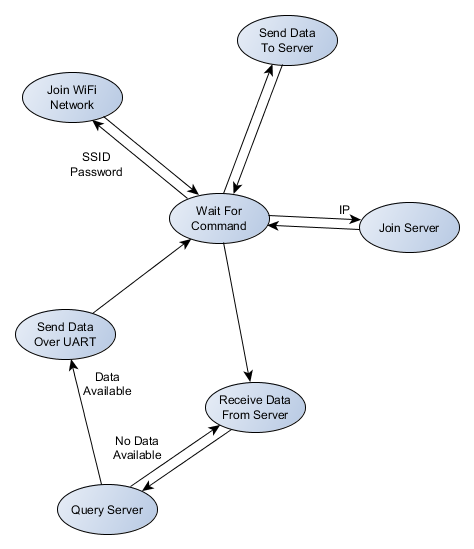
\includegraphics[scale=.5]{WiFi_Module_State}}

\begin{center}
State diagram of the WiFi module system.
\end{center}

\vspace*{5mm}

\section*{Hardware}
\indent

All the peripherals required to run the project, including LCD display, stepper motor drivers, electromagnet, and reed switch array, are interfaced to the microcontroller using general purpose input/output pins. These pins are are software controllable, allowing the software to interface with the hardware. The microcontroller is connected to the WiFi module over a hardware UART bus, which differs from the GPIO's used to control the other peripherals but still allows software control of data between the microcontroller and WiFi module.

\vspace*{5mm}

\centerline{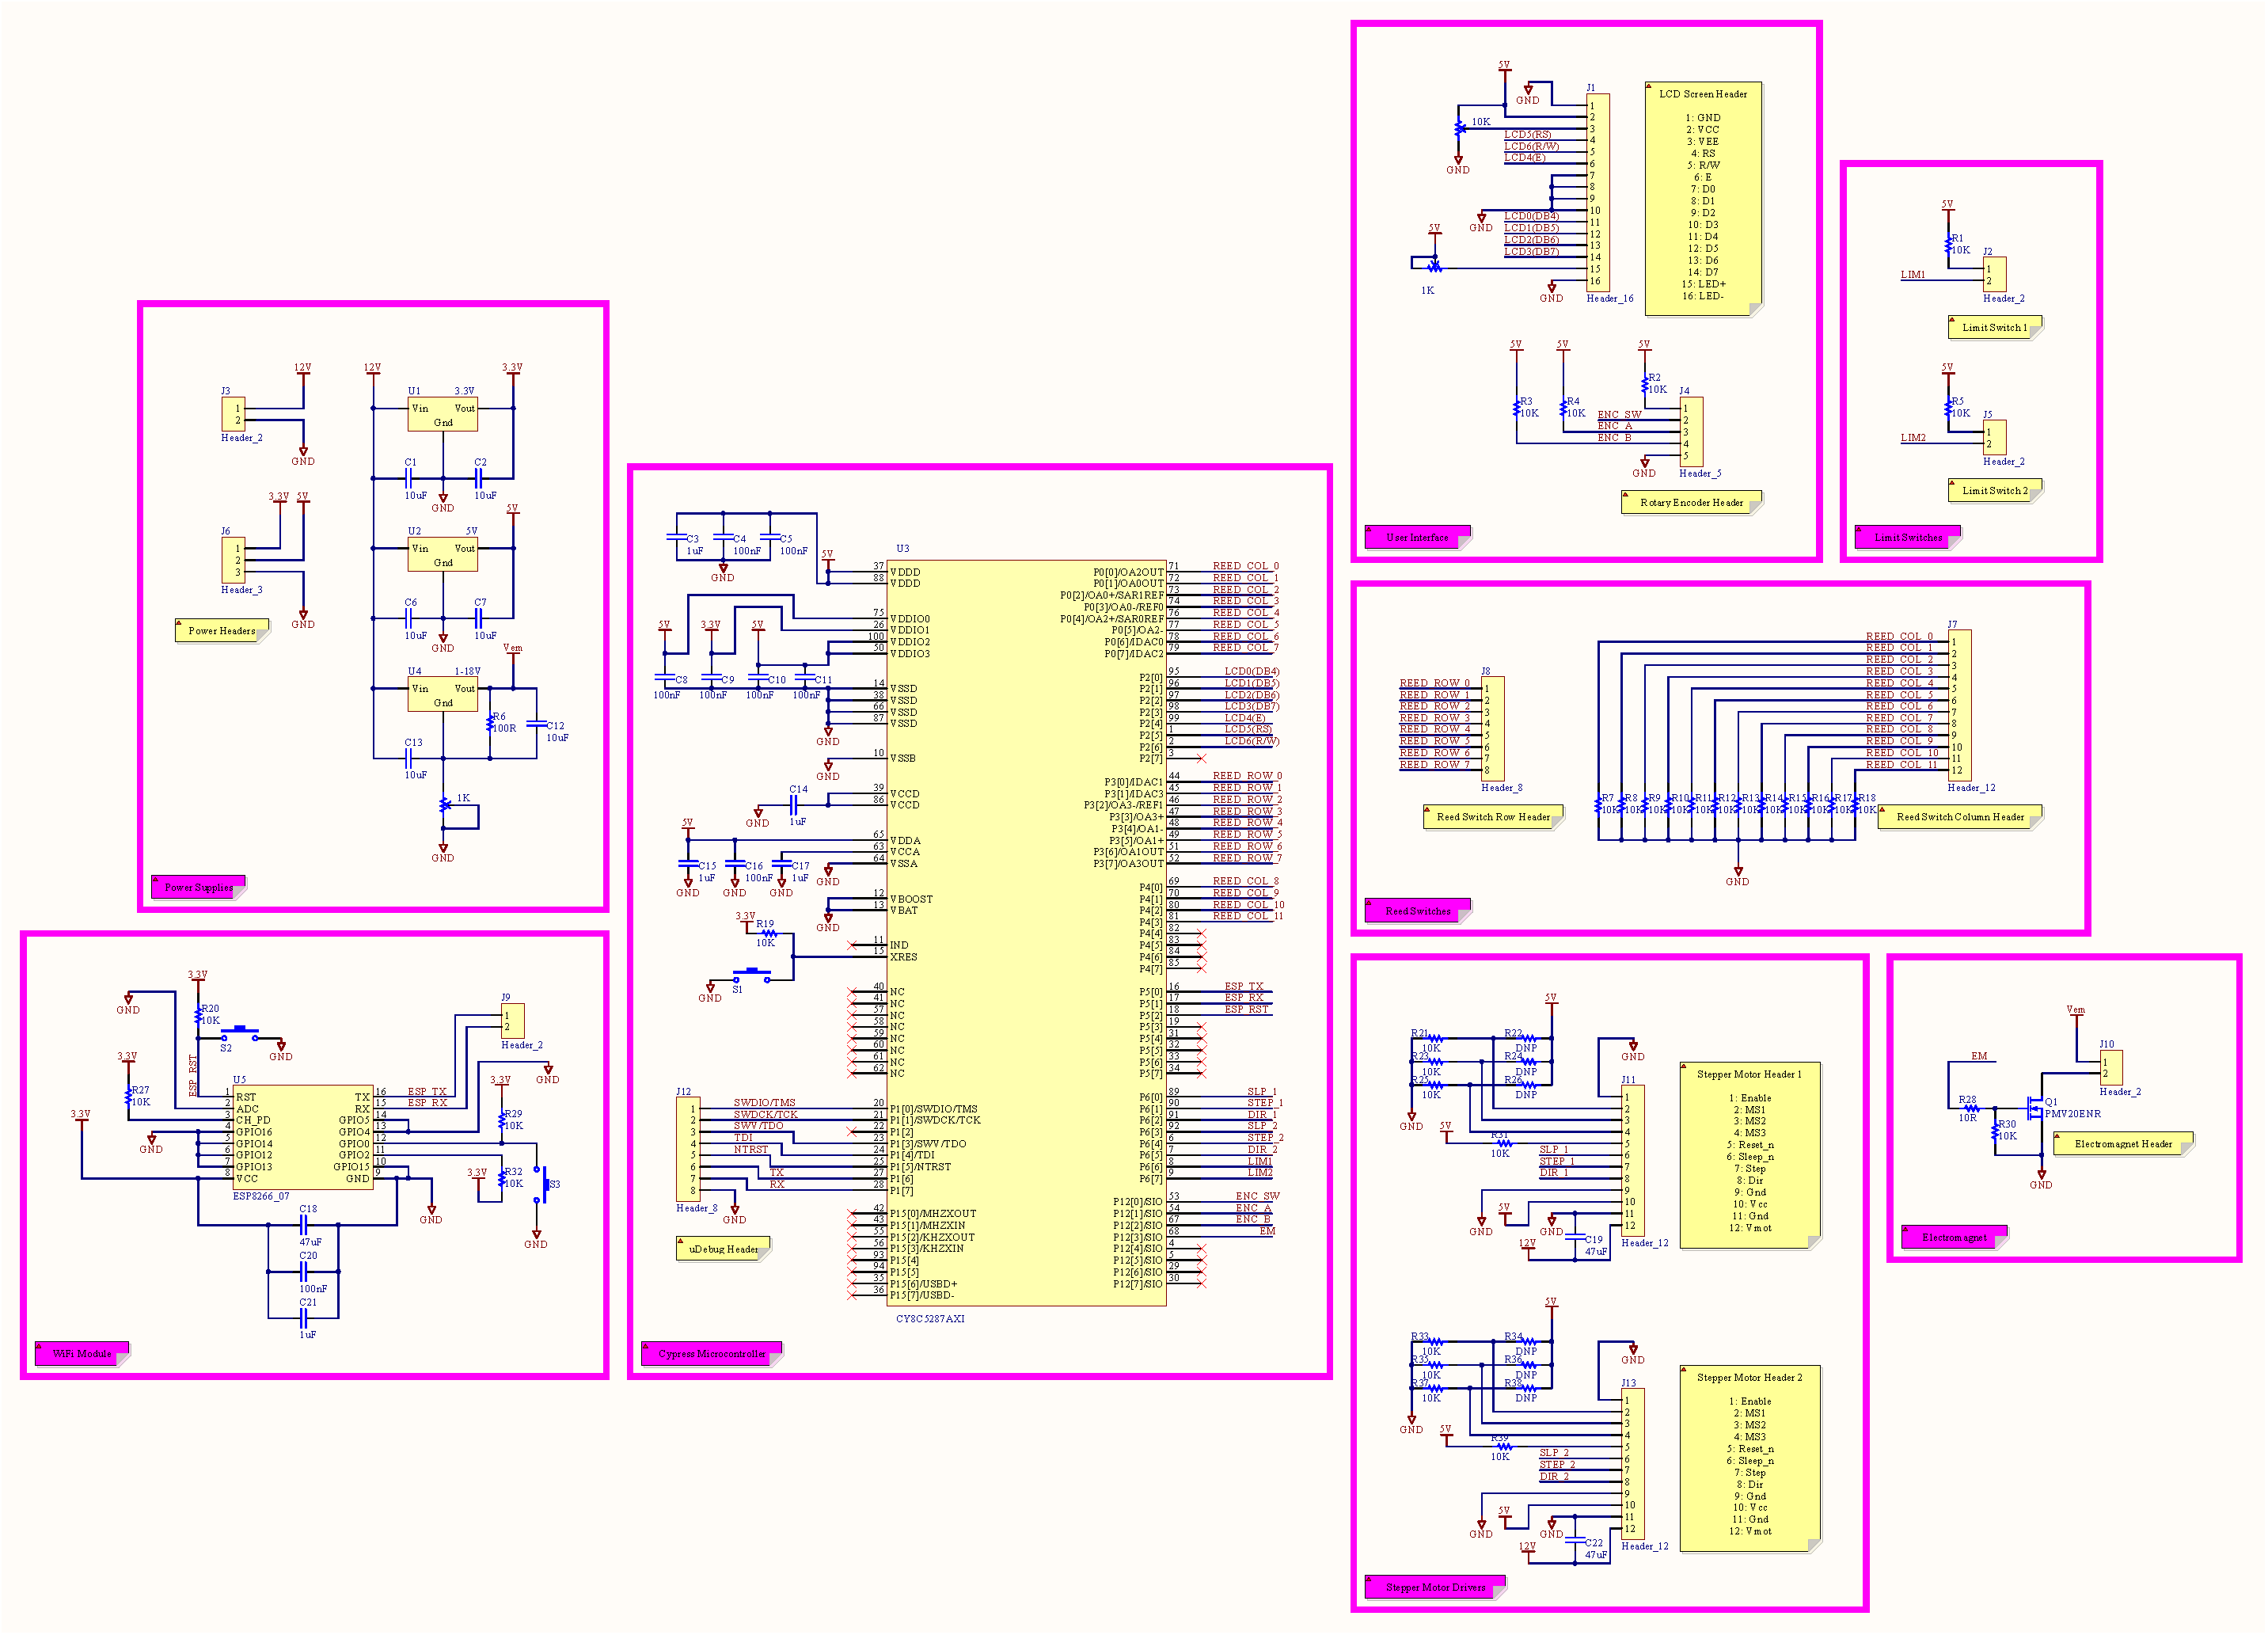
\includegraphics[scale=.5]{Schematic}}

\begin{center}
Schematic of the embedded hardware.
\end{center}

\vspace*{5mm}

\section*{Diagram Information}
\indent

For our project we determined that a UML state diagram would be the most fitting diagram. Because of the both sequential and cyclical nature of the game of chess it would be the most efficient way to represent our systems in graphical form. State diagrams also allow us to show how both players progress through their states at the same time as the other player, giving a sense of where a player would have to wait for his opponent.

\end{document}